\chapter{Summary of Progress}

\section{Data Preparation}

All the datasets necessary for the analysis has been gathered. Most of it has
been downloaded from public sources on the Internet, using Shell and R scripts.
The wind dataset has been provided by Yesubabu Viswanadhapalli, and is the
result of the assimilation of all available atmospheric satellite and in situ
data in the Red Sea into the Weather Research and Forecasting (WRF) regional
Red Sea model. There are additional datasets that will be useful for the
analysis. These are mainly climate mode time-series such as the Indian Monsoon
Index (IMI) and the East Atlantic - West Russian (EAWR) patterns, that are easy
to obtain. The downloaded data is listed and described in table \ref{tab:data}.

So far, the MODIS and CCI data have been cropped over the region of interest,
cleaned and exported to the format TIFF, which can be easily read by most
software, R in particular. Each dataset has then been aggregated in a single
file in the native R raster format. Applying this processing to the remaining
grid data should be straightforward. Then, the data will need to be aligned
and aggregated on the same temporal and spatial resolution, before aggregating
it in table format.

\afterpage{

\thispagestyle{empty}

\begin{landscape}
\begin{table}
\centering 
\begin{tabular}{l c c ccc c} 

\toprule 
Variable & Description             & Mission/Source    & Unit                 & Temporal   & Period & Spatial    \\
         &                         &                   &                      & Resolution &        & Resolution \\
\midrule 

CHL      & Chlorophyll             & CCI               & mg/m${}^3$           & 8-days     & 1997-2012 & 4km   \\
SST      & Sea Surface Temperature & MODIS             & Celsius              & 8-days     & 2002-2015 & 4km   \\
AOD      & Aerosol Optical Depth   & MODIS             & N/A                  & daily      & 2000-2015 & 28km  \\
CDOM     & Colored Dissolved       & MODIS             & N/A                  & 8-days     & 2002-2015 & 4km   \\
         & Organic Matter          &                   &                      &            &           &       \\
NAO      & North Atlantic          & NOAA              & N/A                  & daily      & 1979-2015 &  N/A  \\
         & Oscillation Index       &                   &                      &            &           &       \\
PAR      & Photosynthetically      & MODIS             & Einstein/m${}^2$.Day & 8-days     & 2002-2015 &  4km  \\
         & Available Radiations    &                   &                      &            &           &       \\
POC      & Particulate Organic     & MODIS             & mg/m${}^3$           & 8-days     & 2002-2015 &  4km  \\
         & Carbon                  &                   &                      &            &           &       \\
RAIN     & Precipitations          & TRMM              & mm/h                 & daily      & 1998-2015 & 28km  \\
SOI      & Southern Oscillation    & Australian Bureau & N/A                  & daily      & 1999-2015 &  N/A  \\
         & Index                   & of Meteorology    &                      &            &           &       \\
SLA      & Sea Level Anomaly       & Aviso             & cm                   & daily      & 1993-2013 &  28km \\
WIND     & Vector Wind Field       & Simulated         & m/s                  & 3-hourly   & 2000-2014 &  10km \\

\bottomrule

\end{tabular}
\caption{Downloaded data}
\label{tab:data}
\end{table}
\end{landscape}

\clearpage% Flush page
}



\section{Red Sea Chlorophyll Data Analysis}

The MODIS and CCI chlorophyll data products have been explored and compared.
The MODIS data include an important amount of missing data, which may reach
100\% during summer in the southern Red Sea, increasing the complexity of any
analysis in this region. The CCI data product solves this issue by merging
three sources of remotely-sensed chlorophyll data (MODIS, MERIS and SeaWiFS)
and using a new algorithm for retrieving chlorophyll values when the cloud
cover is important.  This increases the coverage to 70\% during summer months
in the southern Red Sea.

The SeaWiFS chlorophyll data has been used in the submitted companion article
of Chapter 3 (see Appendice B).  The seasonal signal in the data is strong and
has been shown to account for 50\% of the variability. The seasonal anomalies
display a strong spatio-temporal correlation: the temporal correlation of
anomalies is 40\%, whereas two locations at 0.5 degrees apart are nearly 60\%
correlated. Not shown in this article, I also compared the SST and chlorophyll
data, and found an important negative correlation. However, when looking at the
anomalies, the correlation was not significant, suggesting that the causes of
seasonal and interannual variability are distinct.

\section{Red Sea Regional Clustering}

I used clustering algorithms in order to derive the Red Sea eco-regions. These
were applied to monthly log-concentration of chlorophyll. I used SeaWiFS data,
that has been filled using DINEOF. I used the popular K-means, and the Gaussian
Mixture Model (GMM) clustering algorithms.

I found that GMM provides more robust results. With any number of clusters, we
obtain a division of the Red Sea into regions of comparable sizes.  With 5
clusters, the regions (shown in figure \ref{cluster}) are very similar to those identified by
\citet{Raitsos2013}.  Contrary to the purely latitudinal division proposed by
the former, we observe that the separation between clusters is curved at the
position of major Red Sea eddies.  The fact that the curvature is oriented
toward the south suggests that most nutrients propagate northward from the Gulf
of Aden.

\begin{figure}[h]
    \centering
    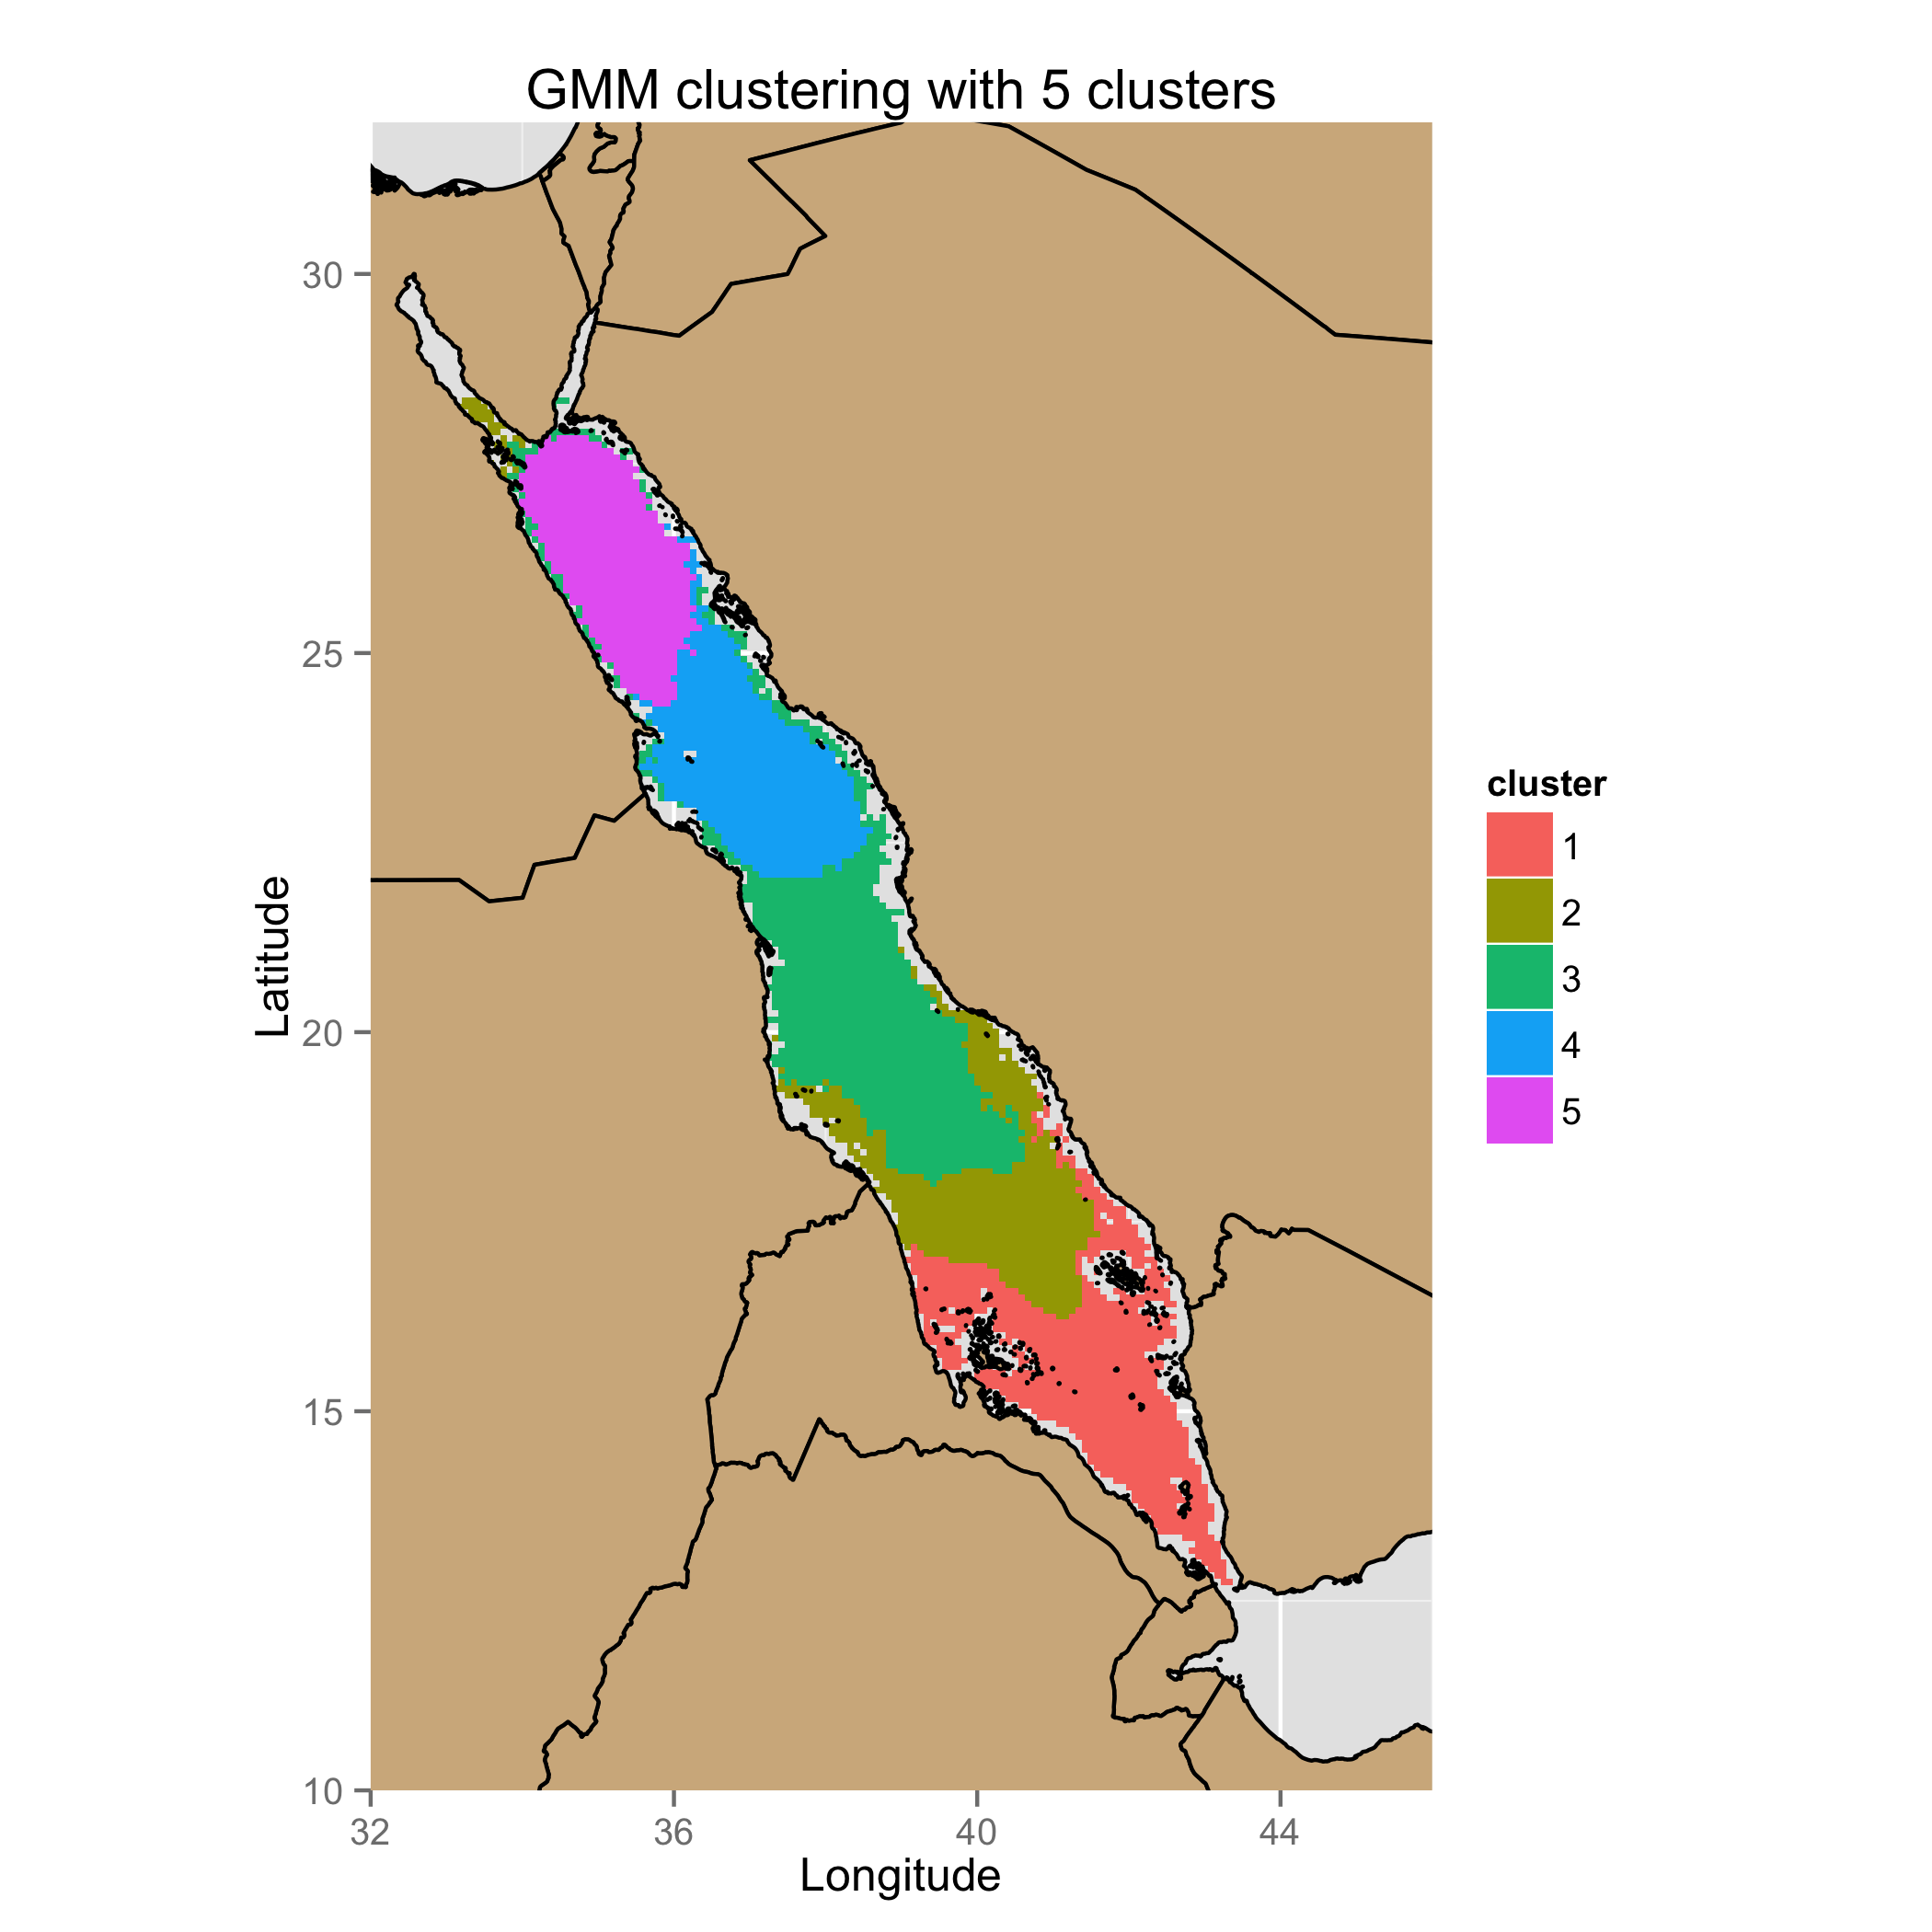
\includegraphics[scale=.15]{figures/clusters_k5.png}
    \caption{Clustering of Red Sea using GMM, with filled monthly SeaWiFS
             chlorophyll data.}
    \label{cluster}
\end{figure}

In Chapter 2, I plan to use the dataset constructed in Chapter 1.  By using CCI
chlorophyll data instead of SeaWiFS, the need for data filling is minimized.
This is desirable, as data filling may introduce biases. It will also be
possible to use additional variables. For example, we can expect the
temperature and the bathymetry to have a large impact on the Red Sea
phytoplankton biology. Sea level anomaly can be useful in that it indicates the
presence of mesoscale eddies. Finally, alternative clustering algorithms will
be tested.

\section{A Global Geostatistical Model}

The research described in Chapter 3 of the thesis has mostly been
done and, is the object of an article currently under review. The current version
of the manuscript can be found in the appendix. We include the abstract below:

\begin{quotation}
\emph{A statistical model is proposed to filter satellite-derived chlorophyll
concentration from the Red Sea, and to predict future chlorophyll
concentrations. The seasonal trend is first estimated after filling missing
chlorophyll data using an Empirical Orthogonal Function (EOF)-based algorithm
(Data Interpolation EOF). The anomalies are then modeled as a stationary
Gaussian process. A method proposed by \citet{Gneiting2002} is used to
construct positive-definite space-time covariance models for this process.
After choosing an appropriate statistical model and identifying its parameters,
Kriging is applied in the space-time domain to make a one step-ahead prediction
of the anomalies. The latter serves as the prediction model of a reduced-order
Kalman filter, which is applied to assimilate and predict future observations
of chlorophyll concentrations. The proposed method decreases the root mean
square (RMS) prediction error by about 11\% compared with the seasonal
prediction.}
\end{quotation}

\section{Regional 1D Ecological Models}

The 1D regional ecological models have been configured and
are operational. Three models will be used: for the northern, central and
southern Red Sea. The extreme south of the Red Sea is not modeled, as its
dynamics is poorly understand and no in situ data are available to validate the
satellite products. The ecology is modeled with ERSEM, and the hydrodynamics
is modeled with the MITgcm.

The physical forcing from the MITgcm are those of \citet{Yao2014, Yao2014b}, in
which a simulation of the Red Sea and part of the Gulf of Aden circulation was
run over 50 years. The NCEP data were used for atmospheric forcing, and the
ocean ECCO data for the open boundary conditions in the Gulf of Aden. The
output of the 50 years run are used for the temperature and vertical
circulation at the modeled points.

ERSEM simulates the complete water column with the pelagic and benthic
ecosystems, as well a their coupling. The equations model the flow of carbon,
nitrogen, phosphorus and silicon in the ecosystem. Living organisms are modeled
in terms of population processes (growth and mortality) and physiological
processes (ingestion, respiration, excretion, and egestion). The biota is
divided into functional groups according to their trophic levels: producers
(phytoplankton), consumers (zooplankton) and decomposers (bacteria), and
further subdivided according to their sizes \citep{Baretta1995}.

The ecological models are initialized from the results of a 3D ecological
simulation of the Red Sea \citep{Triantafyllou2014}. The nutrient
concentrations are initialized using values from the World Ocean Atlas 2005
(WOA 2005). We show the model outputs for the northern Red Sea (Figure
\ref{chl2}), the central Red Sea (Figure \ref{chl1}), and the southern Red Sea
(Figure \ref{chl3}). The models are able to reproduce the seasonality of
chlorophyll concentration, with high values in winter and lower values in the
summer. As noticed in \citet{Raitsos2013}, the winter blooms are associated
with deep mixing, particularly in the northern Red Sea.  During summer, there
is a subsurface chlorophyll maximum in the three regions.

\begin{figure}
    \centering
    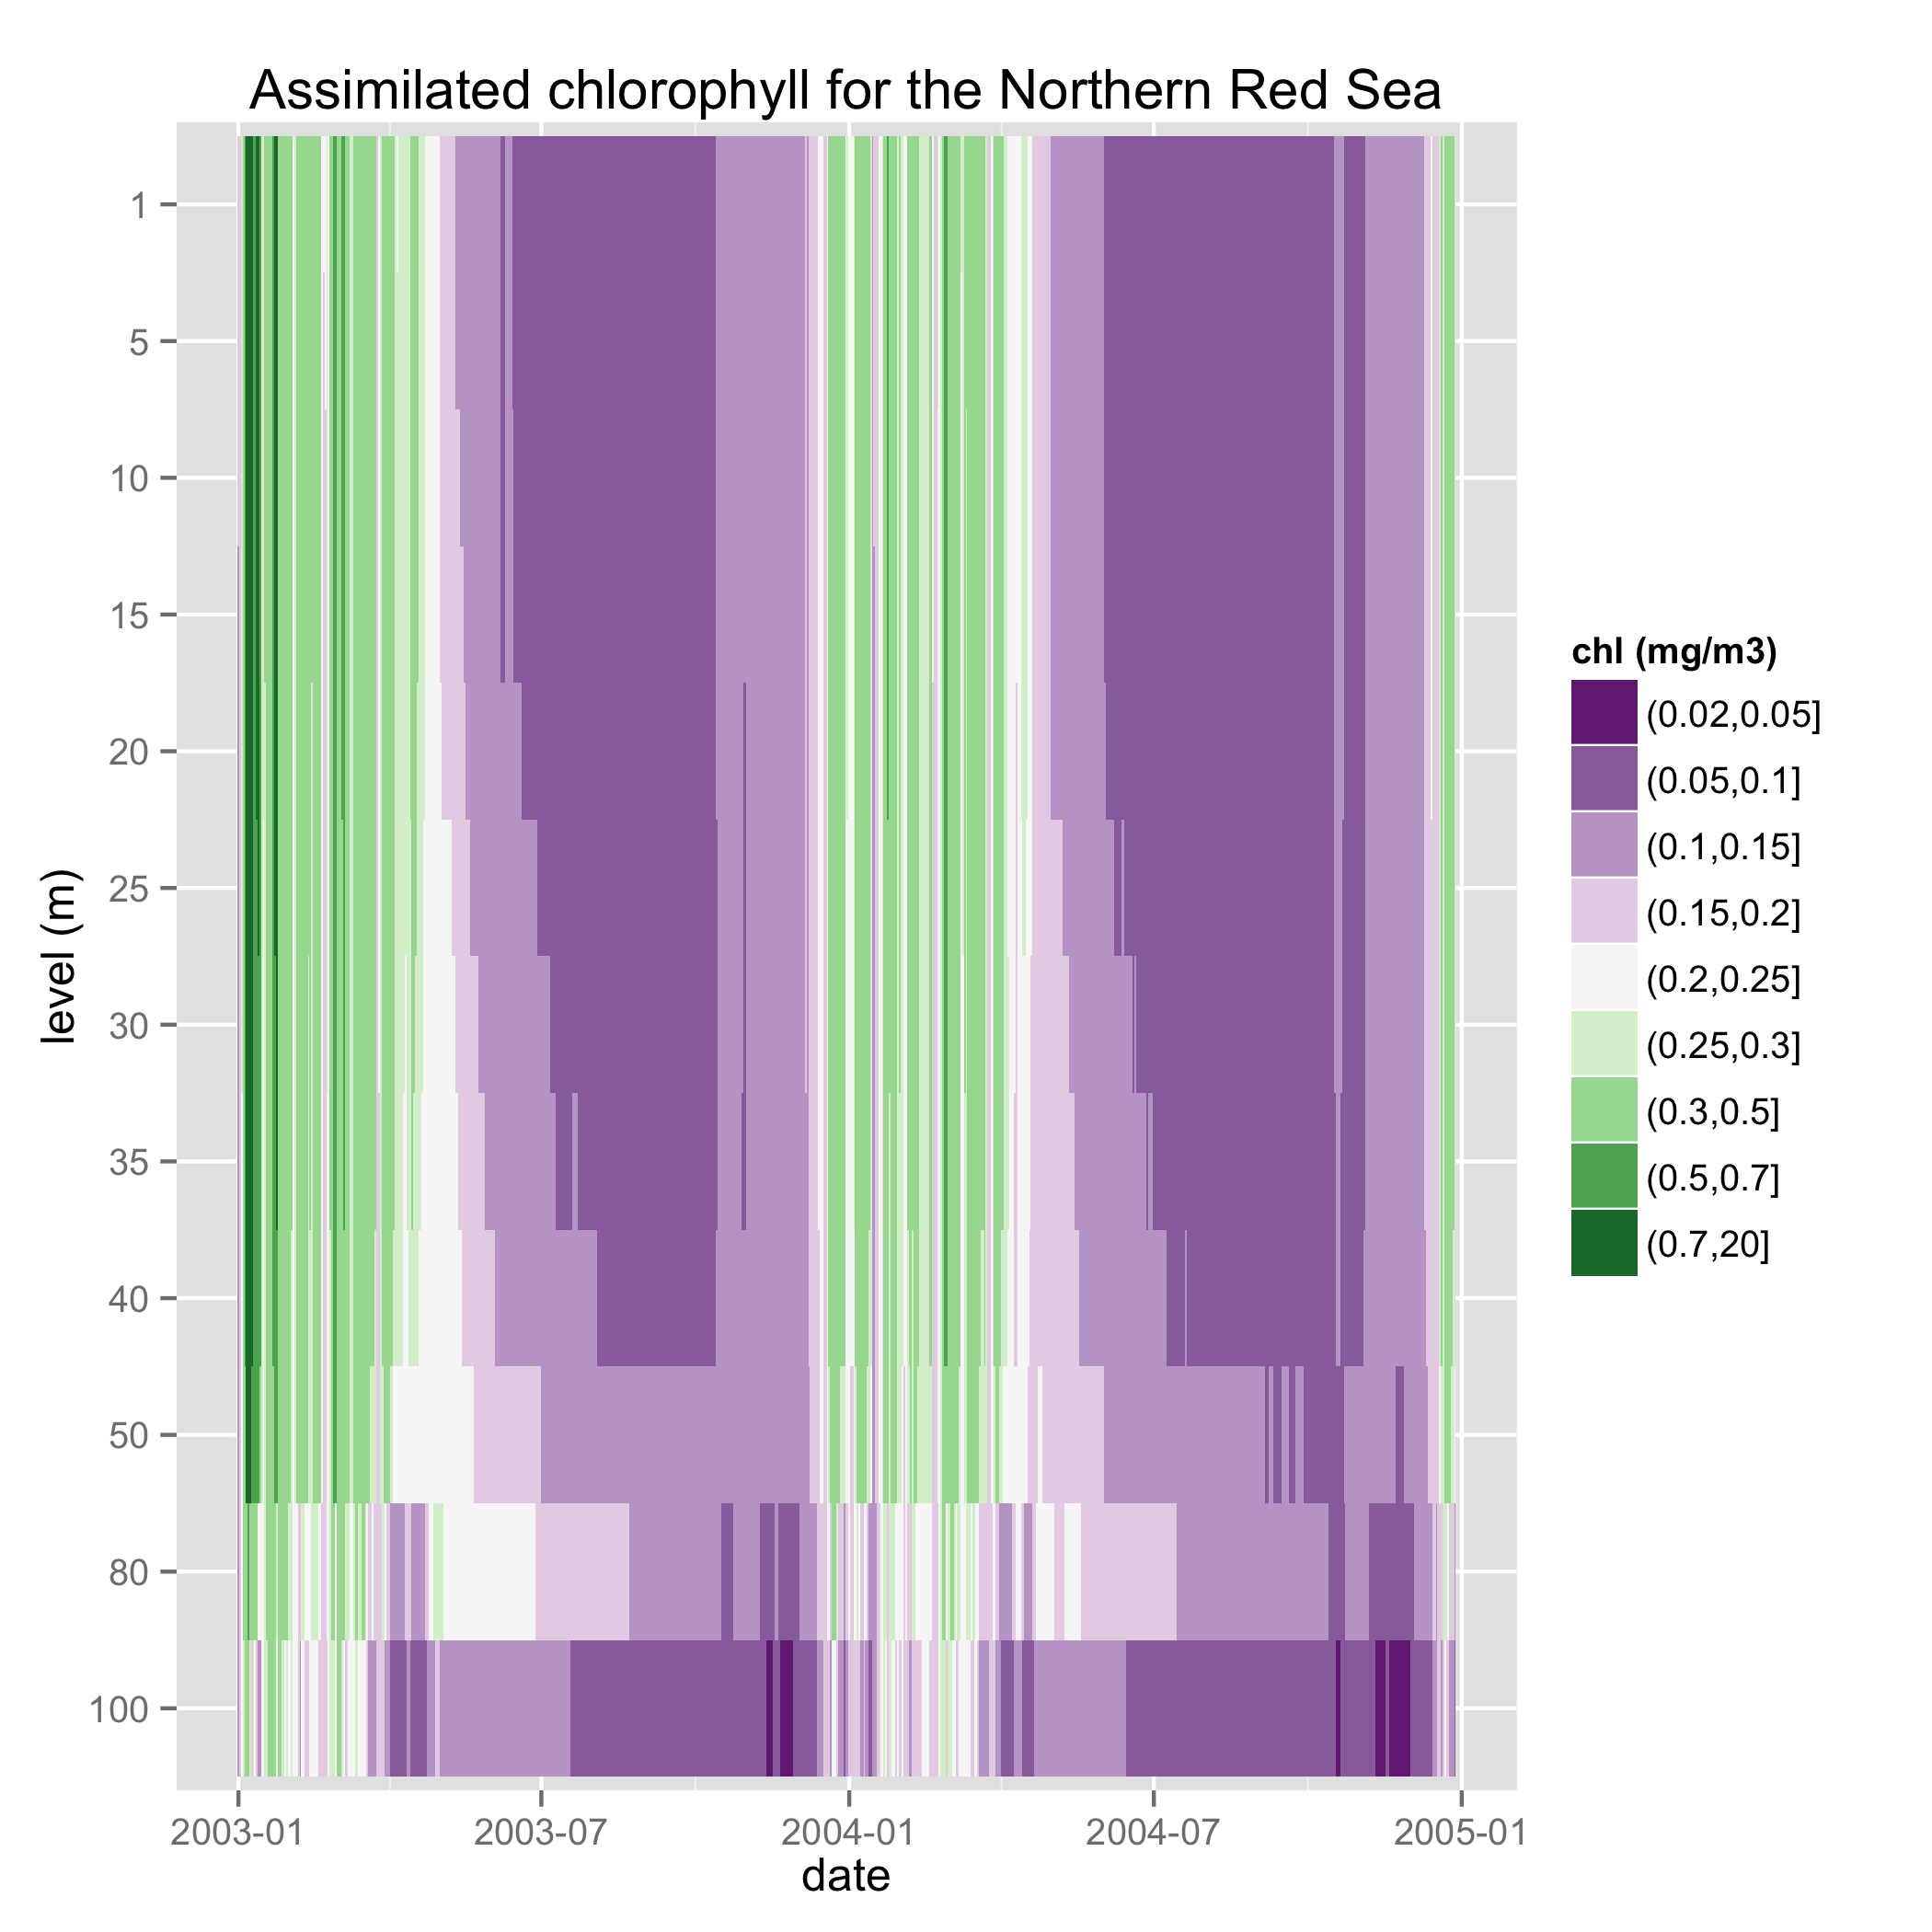
\includegraphics[scale=.13]{figures/chl2.png}
    \caption{Assimilated chlorophyll in the northern Red Sea}
    \label{chl2}
\end{figure}

\begin{figure}
    \centering
    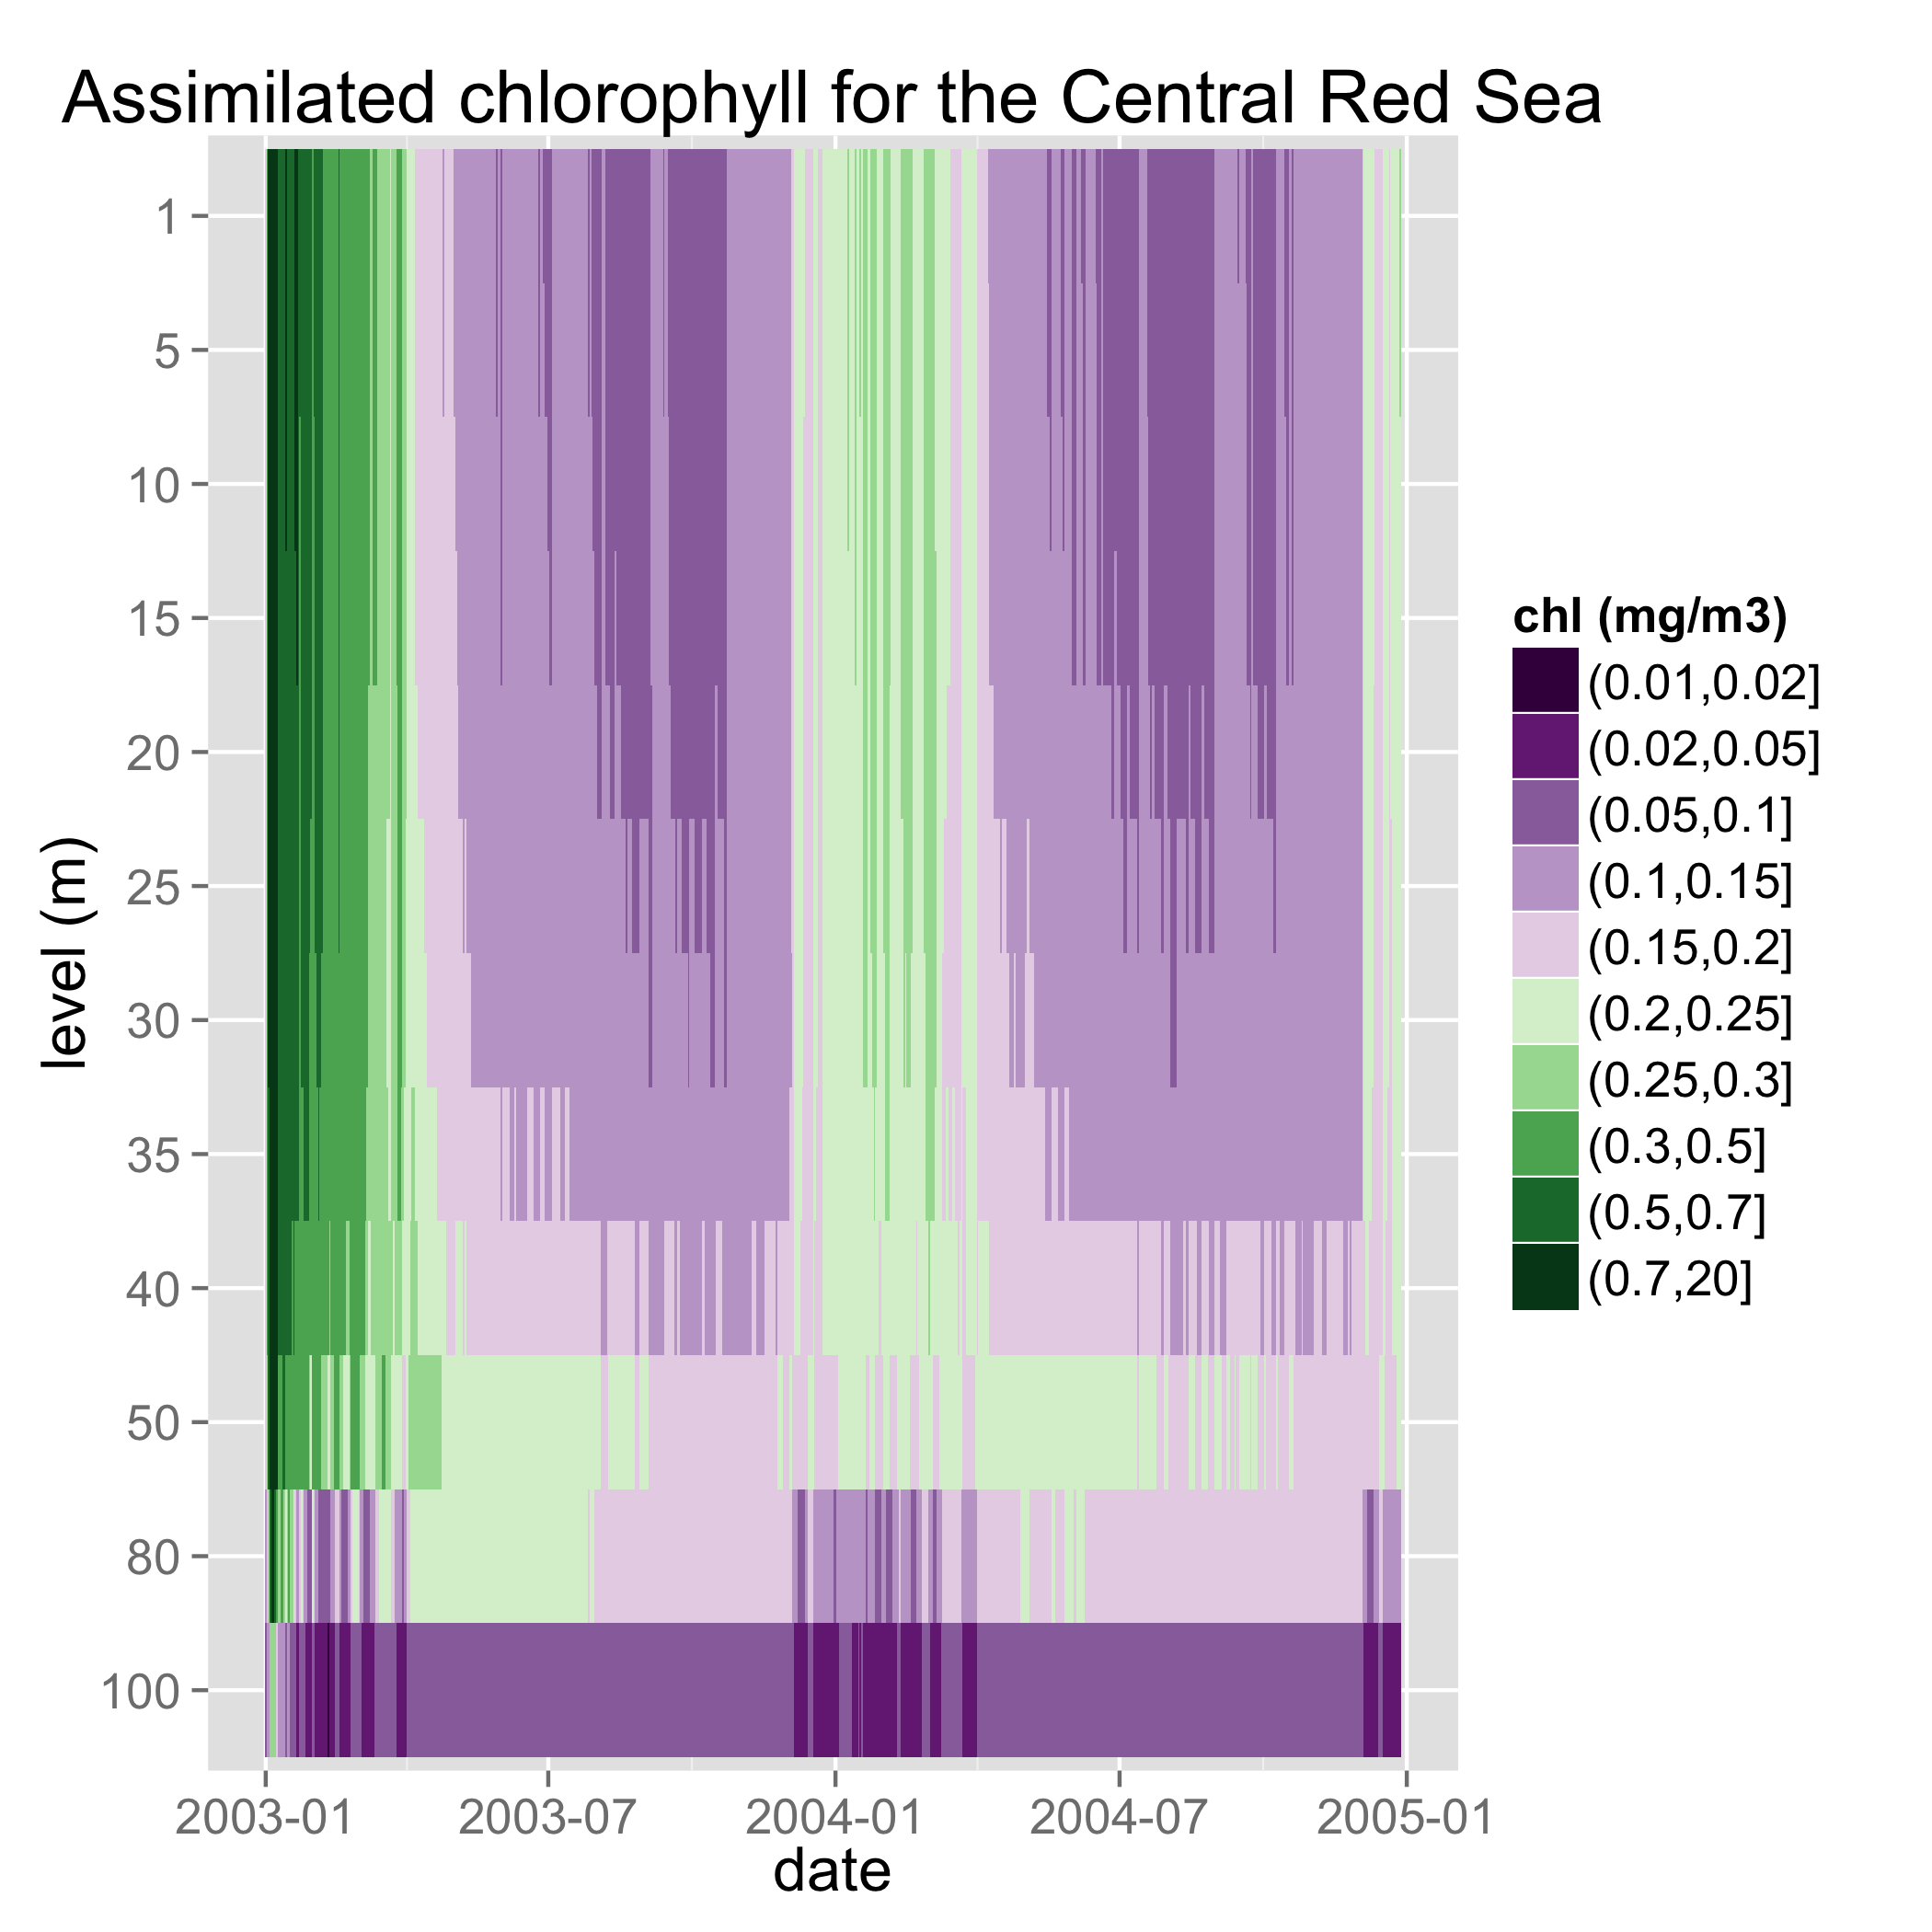
\includegraphics[scale=.13]{figures/chl1.png}
    \caption{Assimilated chlorophyll in the central Red Sea}
    \label{chl1}
\end{figure}

\begin{figure}
    \centering
    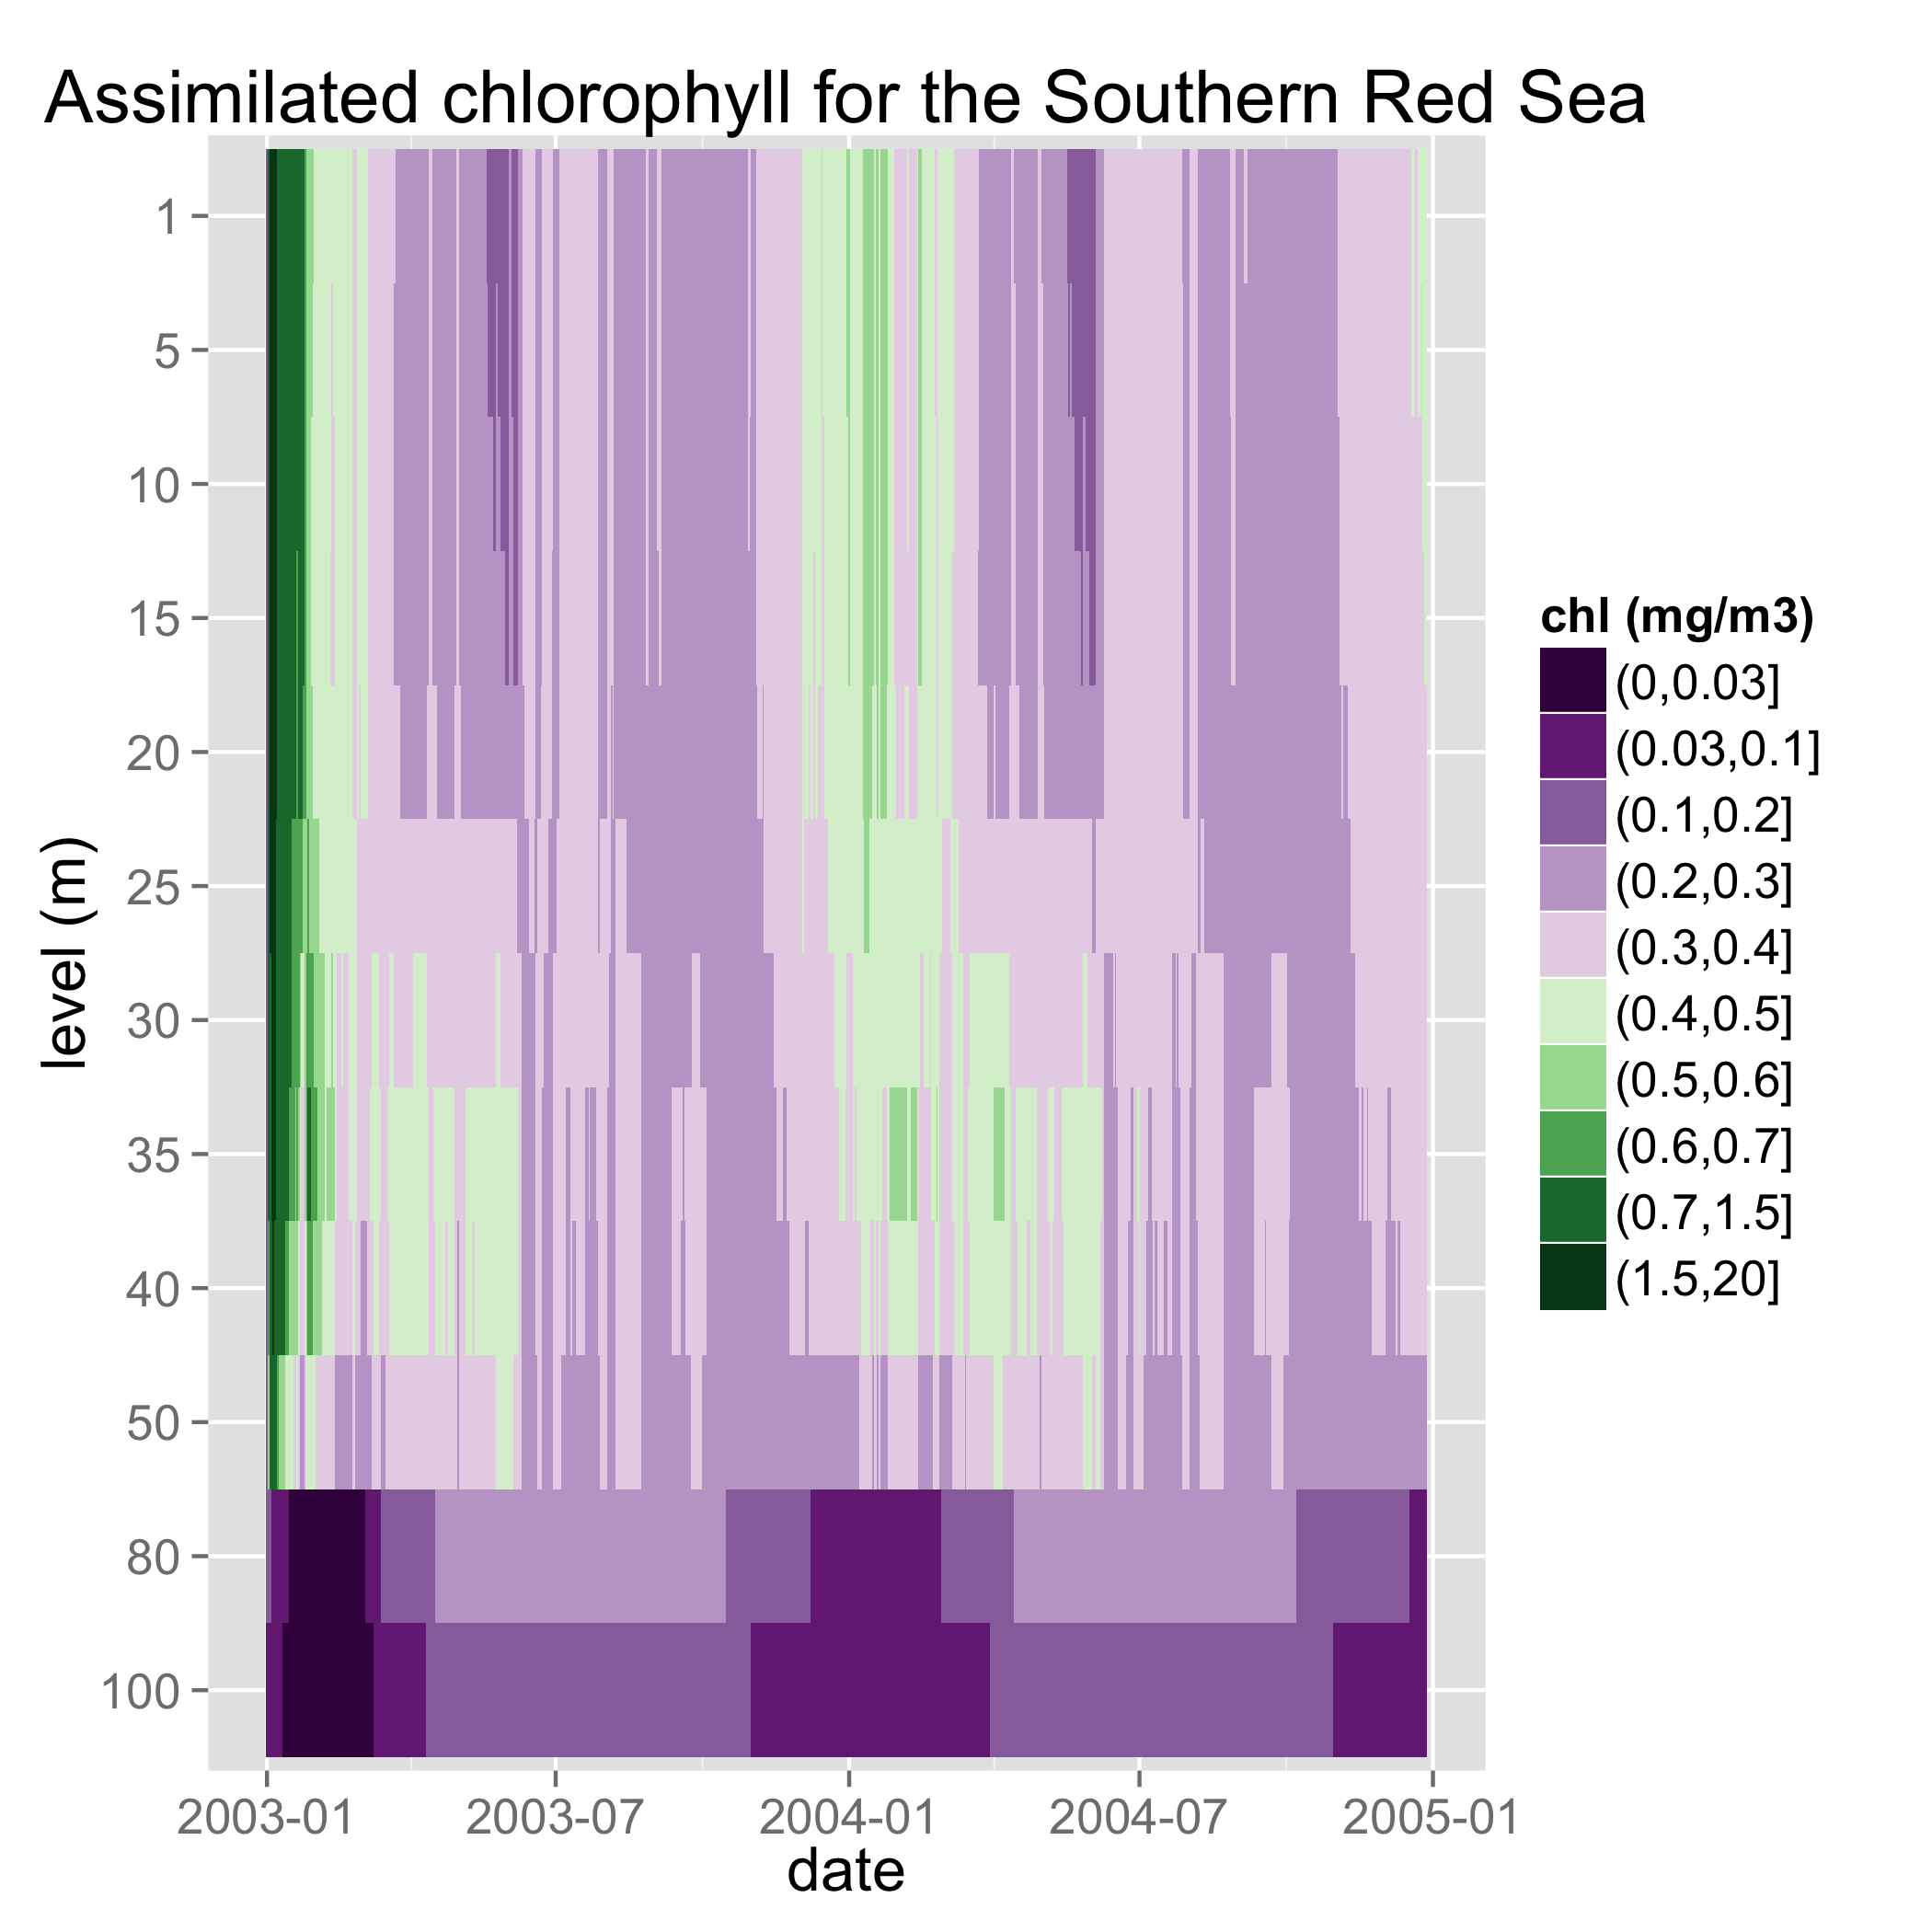
\includegraphics[scale=.13]{figures/chl3.png}
    \caption{Assimilated chlorophyll in the southern Red Sea}
    \label{chl3}
\end{figure}

\section{Data Assimilation into 1D Ecological Models}

The assimilation scheme for the ecological models has been implemented and is
operational. The chosen scheme is a hybrid-SEIK, with the hybrid approach
implemented as described in \citet{Hamill2000}.  The scheme is called hybrid as
it combines the flow-dependent background estimates from the ensemble of an
EnKF with as static background, taken for example from a three-dimensional
variational 3DVAR system. The idea behind it is to complete the rank-deficient
EnKF background by another background that has been designed to capture the
climatological variability of the system.  In our hybrid implementation, the
covariance is a linear combination of the 3DVAR covariance and the
time-evolving SEIK covariance matrix.

The problem of optimal filtering can be solved exactly by the Kalman Filter for
linear systems. For nonlinear models, one can use the Extended Kalman (EK)
filter, in which the model is linearized by computing the error covariance
function.  However, when the state is large, as is often the case for
oceanographic applications, the EK is intractable. In that case, SEEK can be
used, where the error covariance function is projected into a smaller subspace.
This subspace evolves to ensure that most of the error is represented and
filtered out. SEIK can be viewed as an ensemble variant of the SEEK, where the
error covariance function is represented exactly by an ensemble of states. This
avoids the computation of model gradients, and allows the assimilation scheme
to perform better when this model is strongly non-linear. SEIK has been shown
to be efficient for large-scale 3D ecosystem data assimilation
\citep{Triantafyllou2003}.

We show the chlorophyll surface concentration predicted by the models (with and
without assimilation), and the satellite measurements in the three regions in
Figures \ref{chl_models2}, \ref{chl_models1} and \ref{chl_models3}.  The models
reproduce the seasonality of the chlorophyll concentration with low
concentrations in the summer, and a winter bloom. However, the model tends to
overestimate the chlorophyll concentration in winter in the northern Red Sea,
and to underestimate it in the summer in the southern and central Red Sea.
Furthermore, the summer bloom in the southern Red Sea is not well predicted.
However, the assimilation is able to correct these biases, and leads to better
estimates of chlorophyll concentration.

\begin{figure}
    \centering
    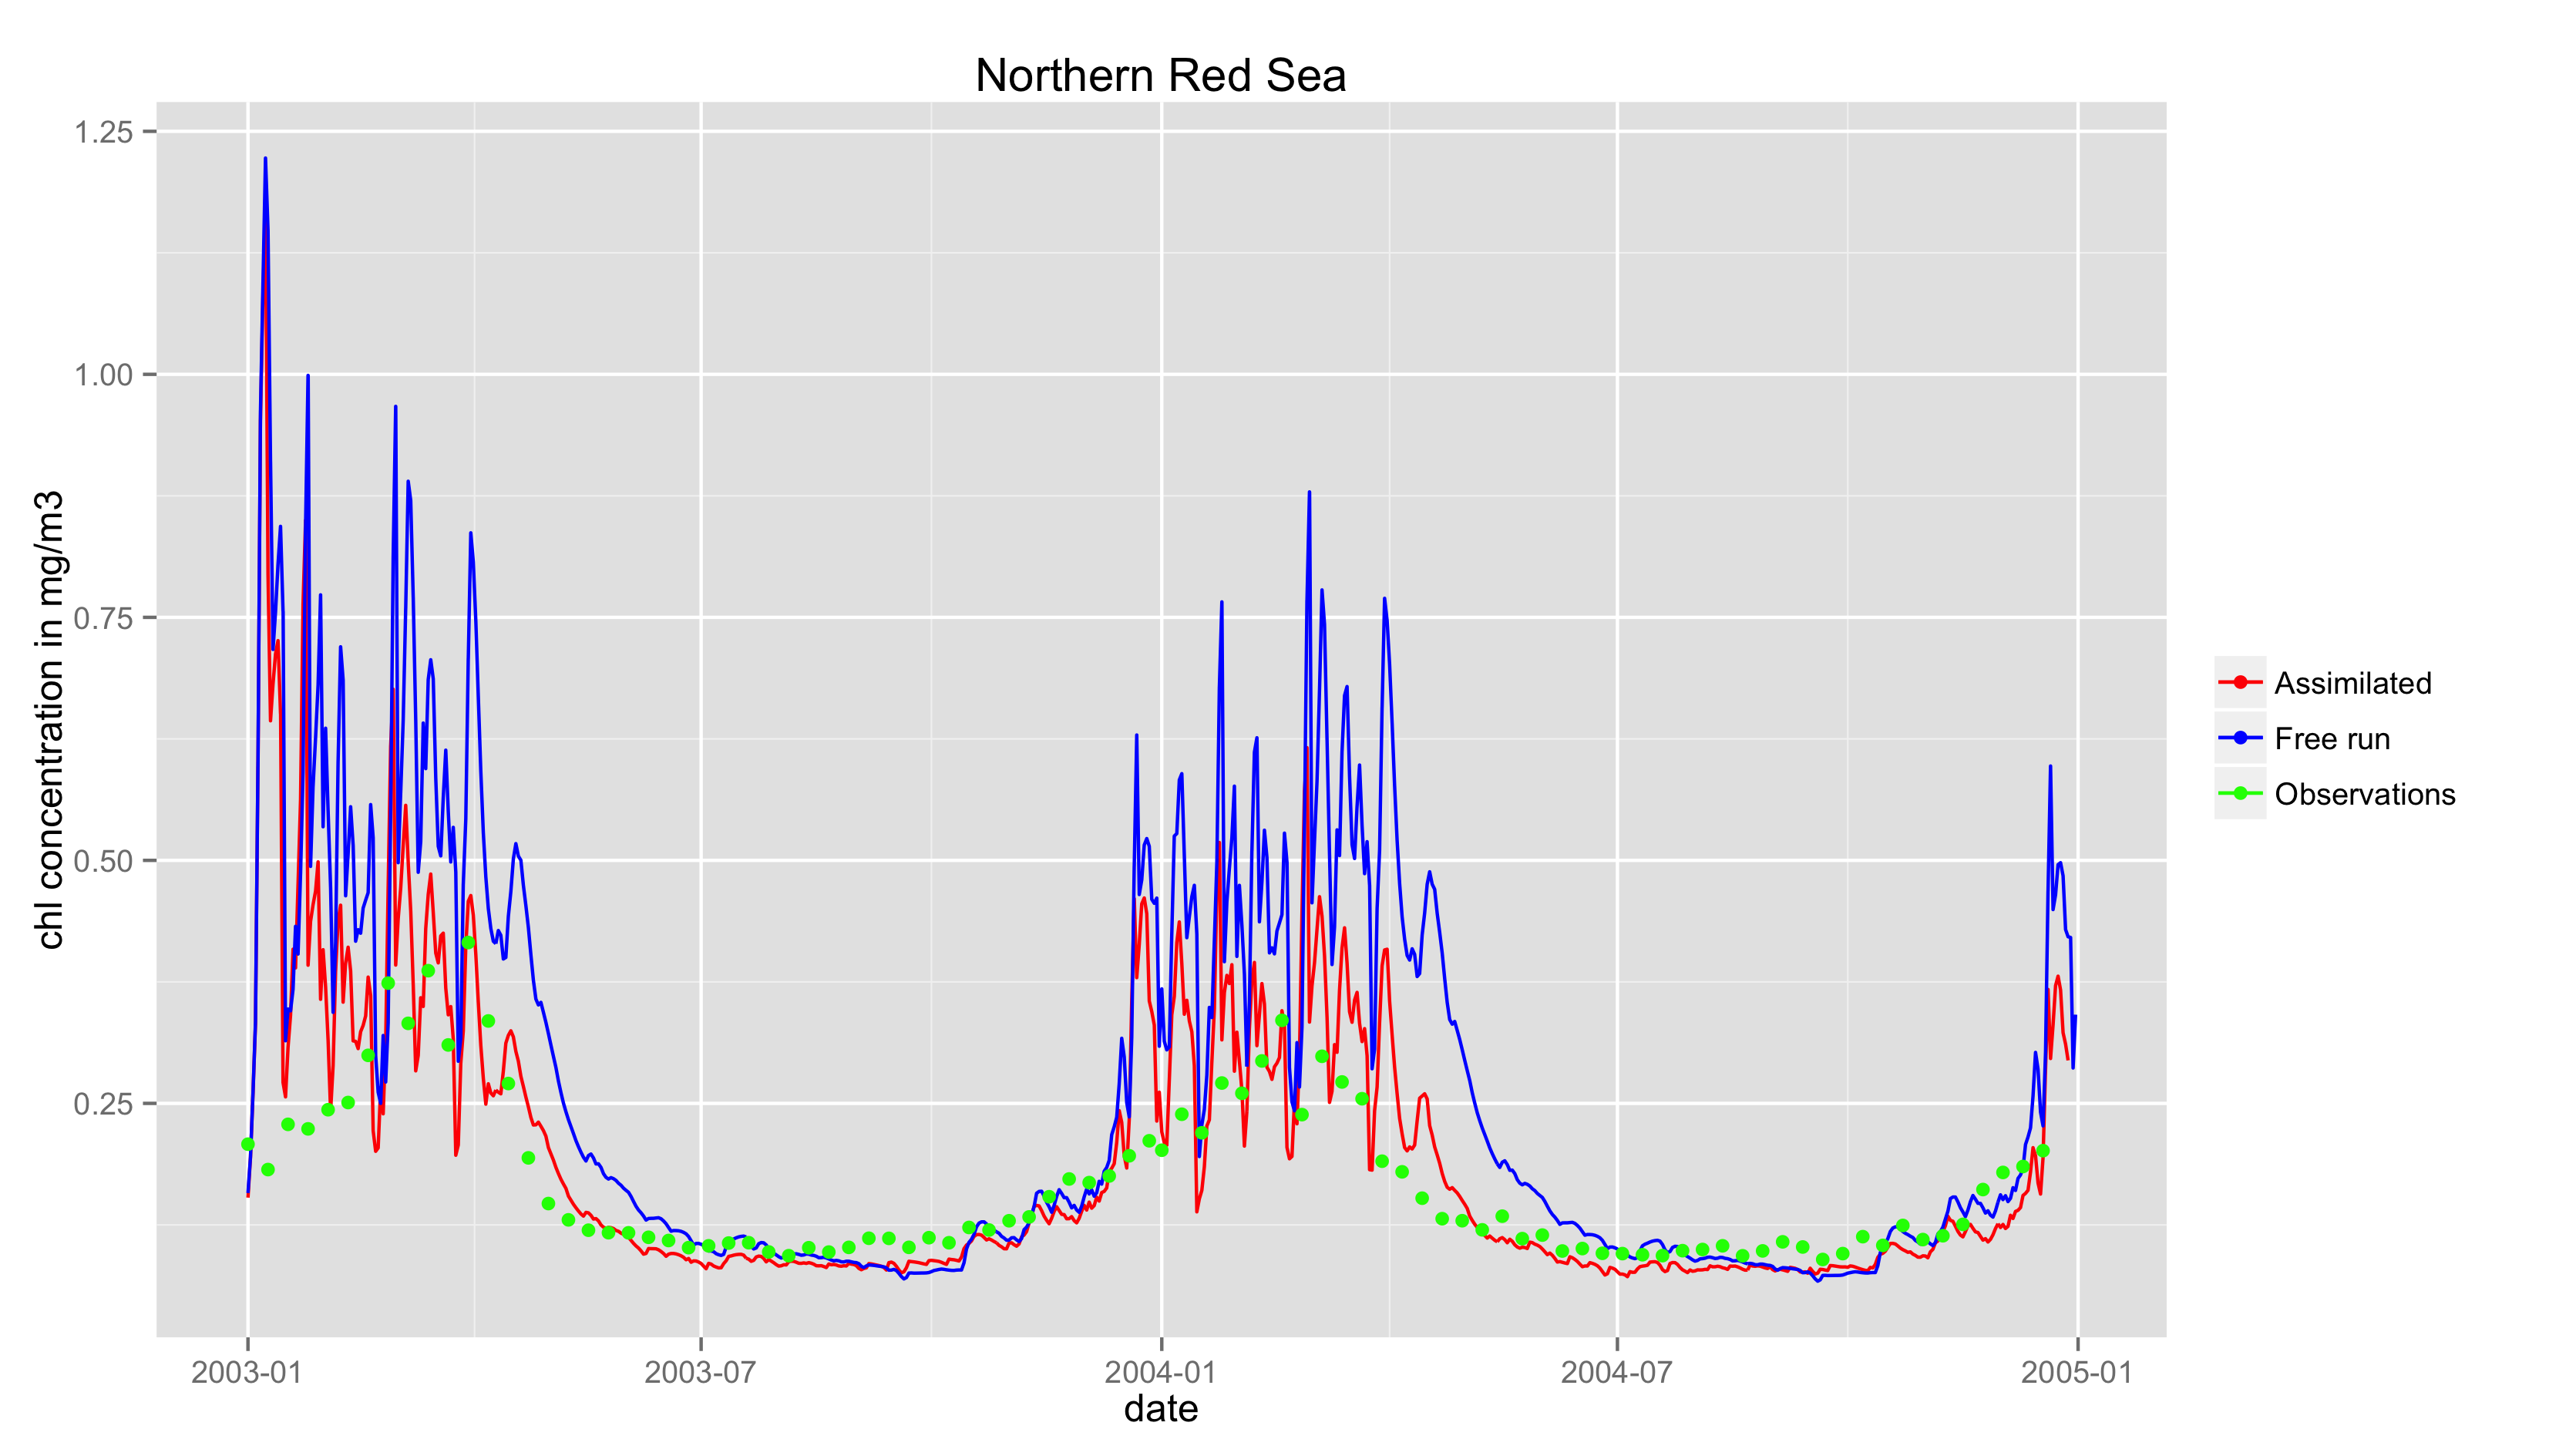
\includegraphics[scale=.15]{figures/chl_models2.png}
    \caption{Surface chlorophyll in the northern Red Sea from CCI data,
             assimilated, and non assimilated 1D ecological model}
    \label{chl_models2}
\end{figure}

\begin{figure}
    \centering
    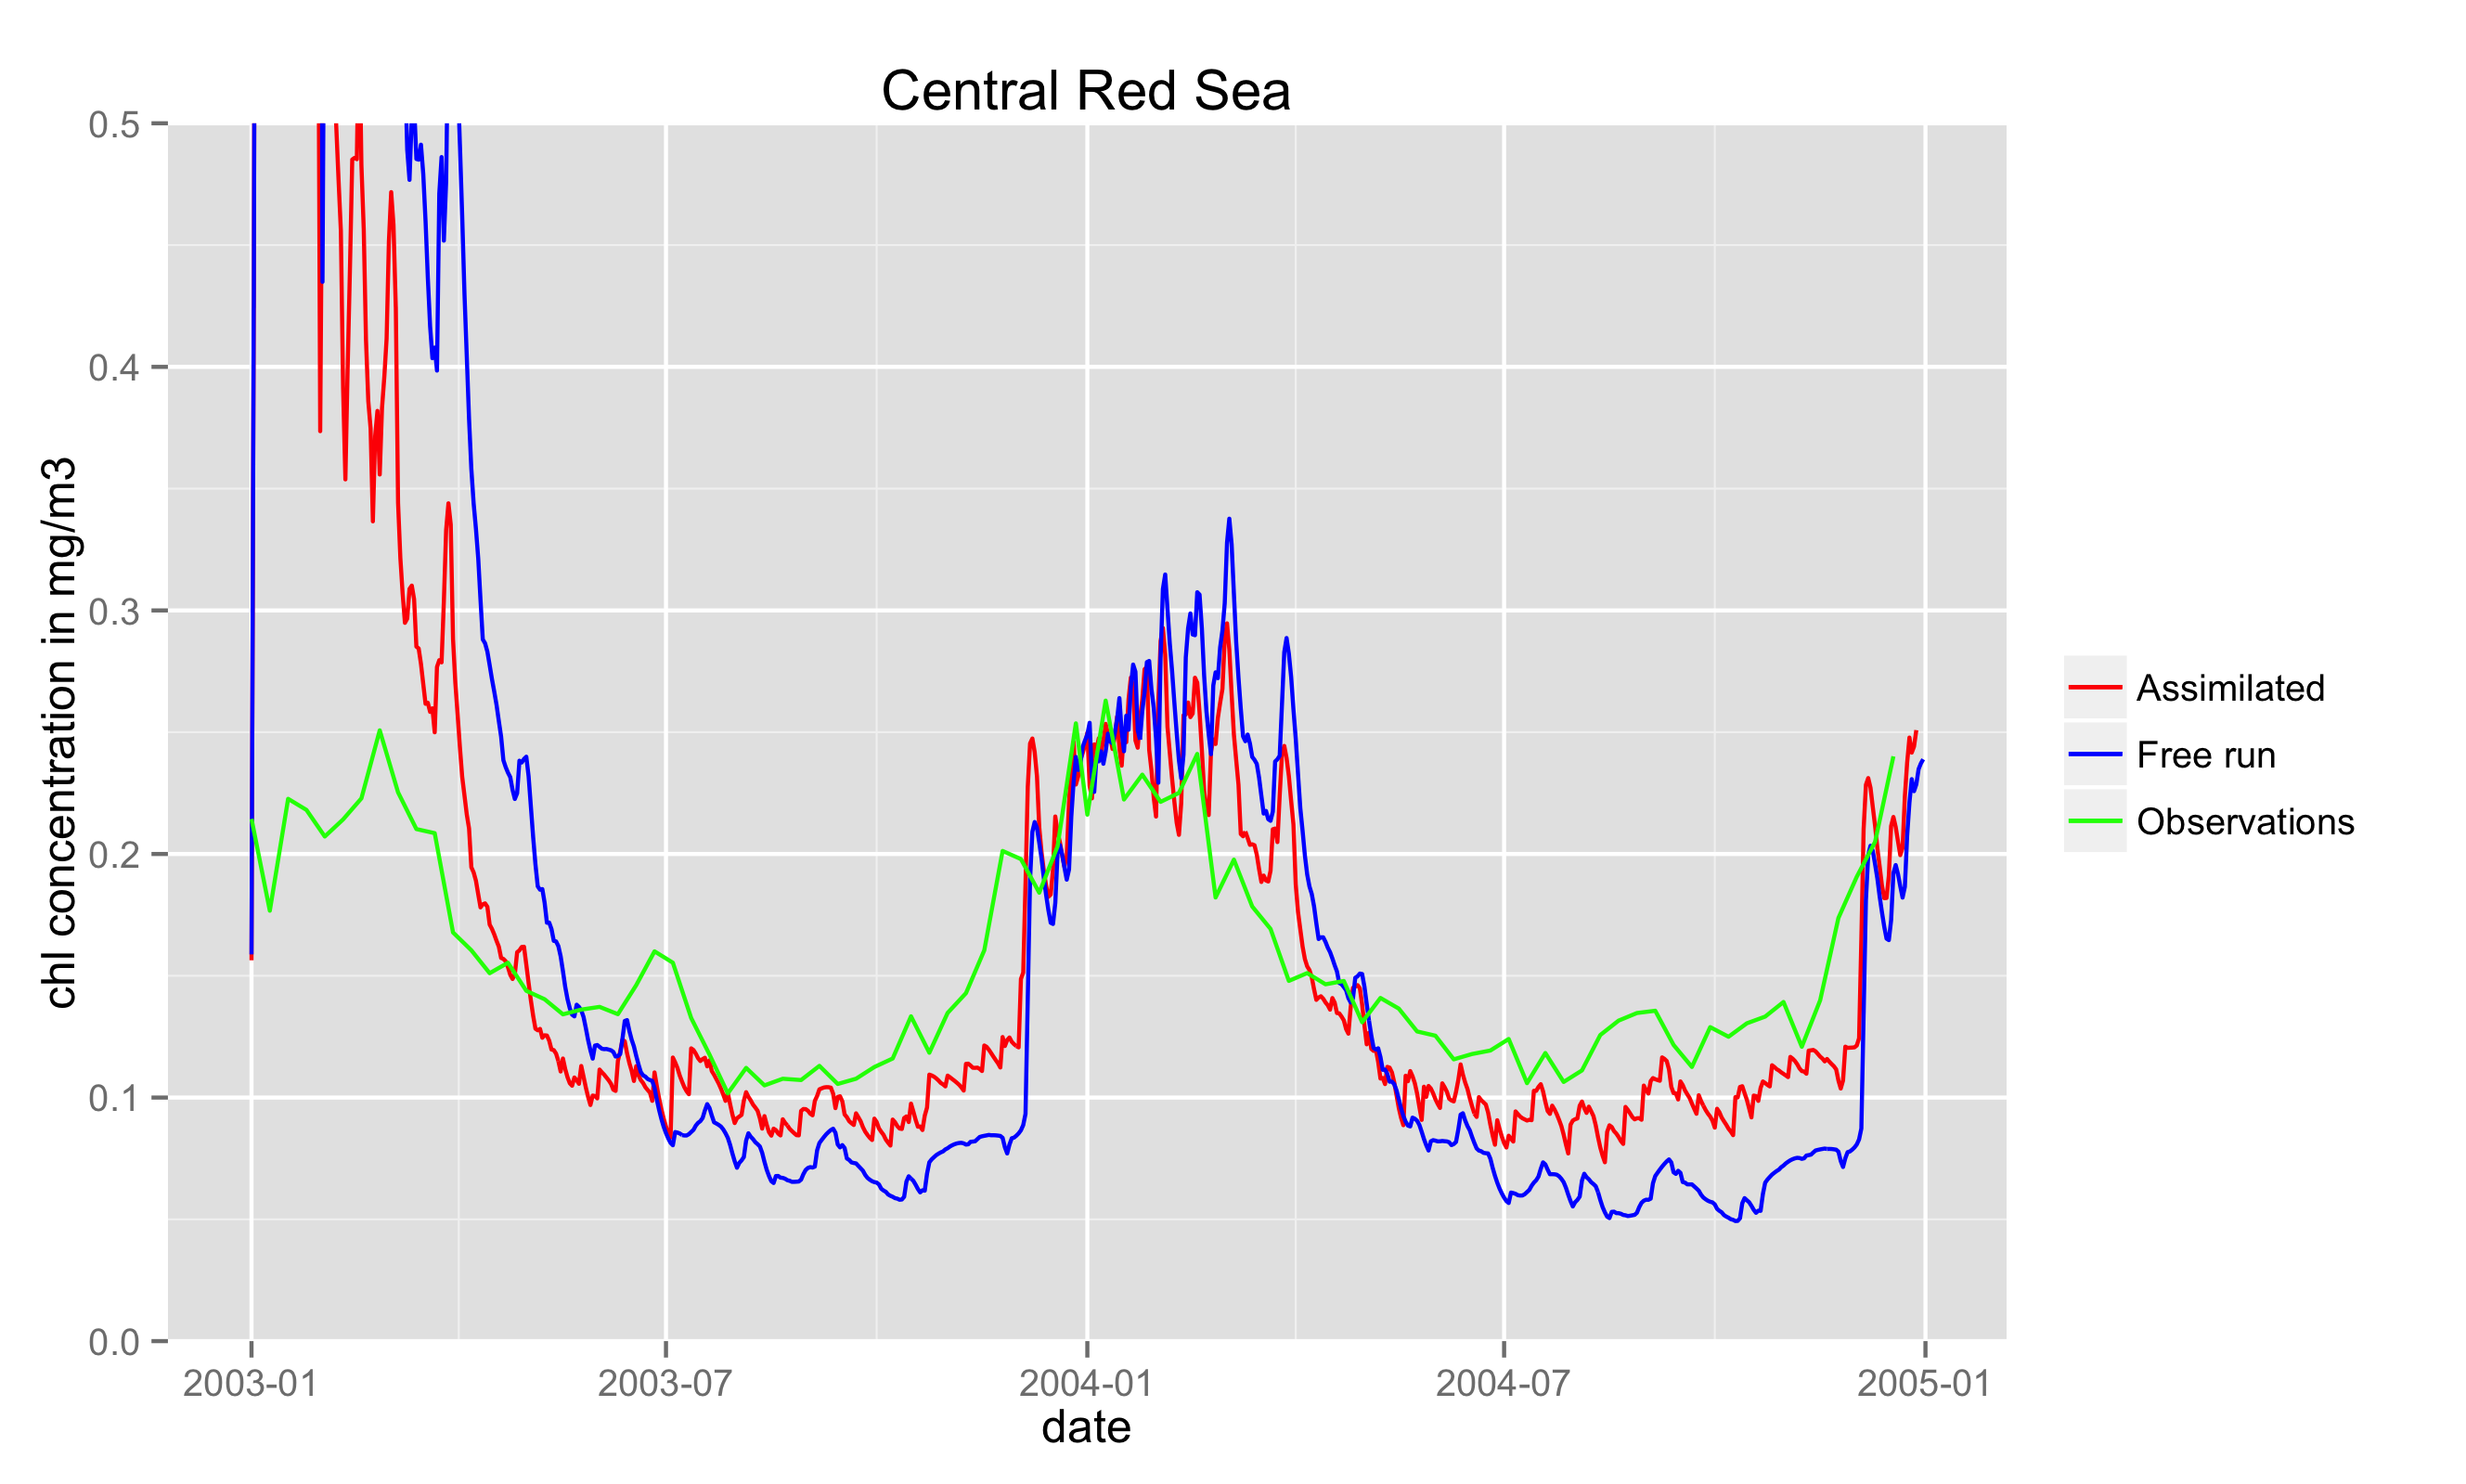
\includegraphics[scale=.15]{figures/chl_models1.png}
    \caption{Surface chlorophyll in the central Red Sea from CCI data,
             assimilated, and non assimilated 1D ecological model}
    \label{chl_models1}
\end{figure}

\begin{figure}
    \centering
    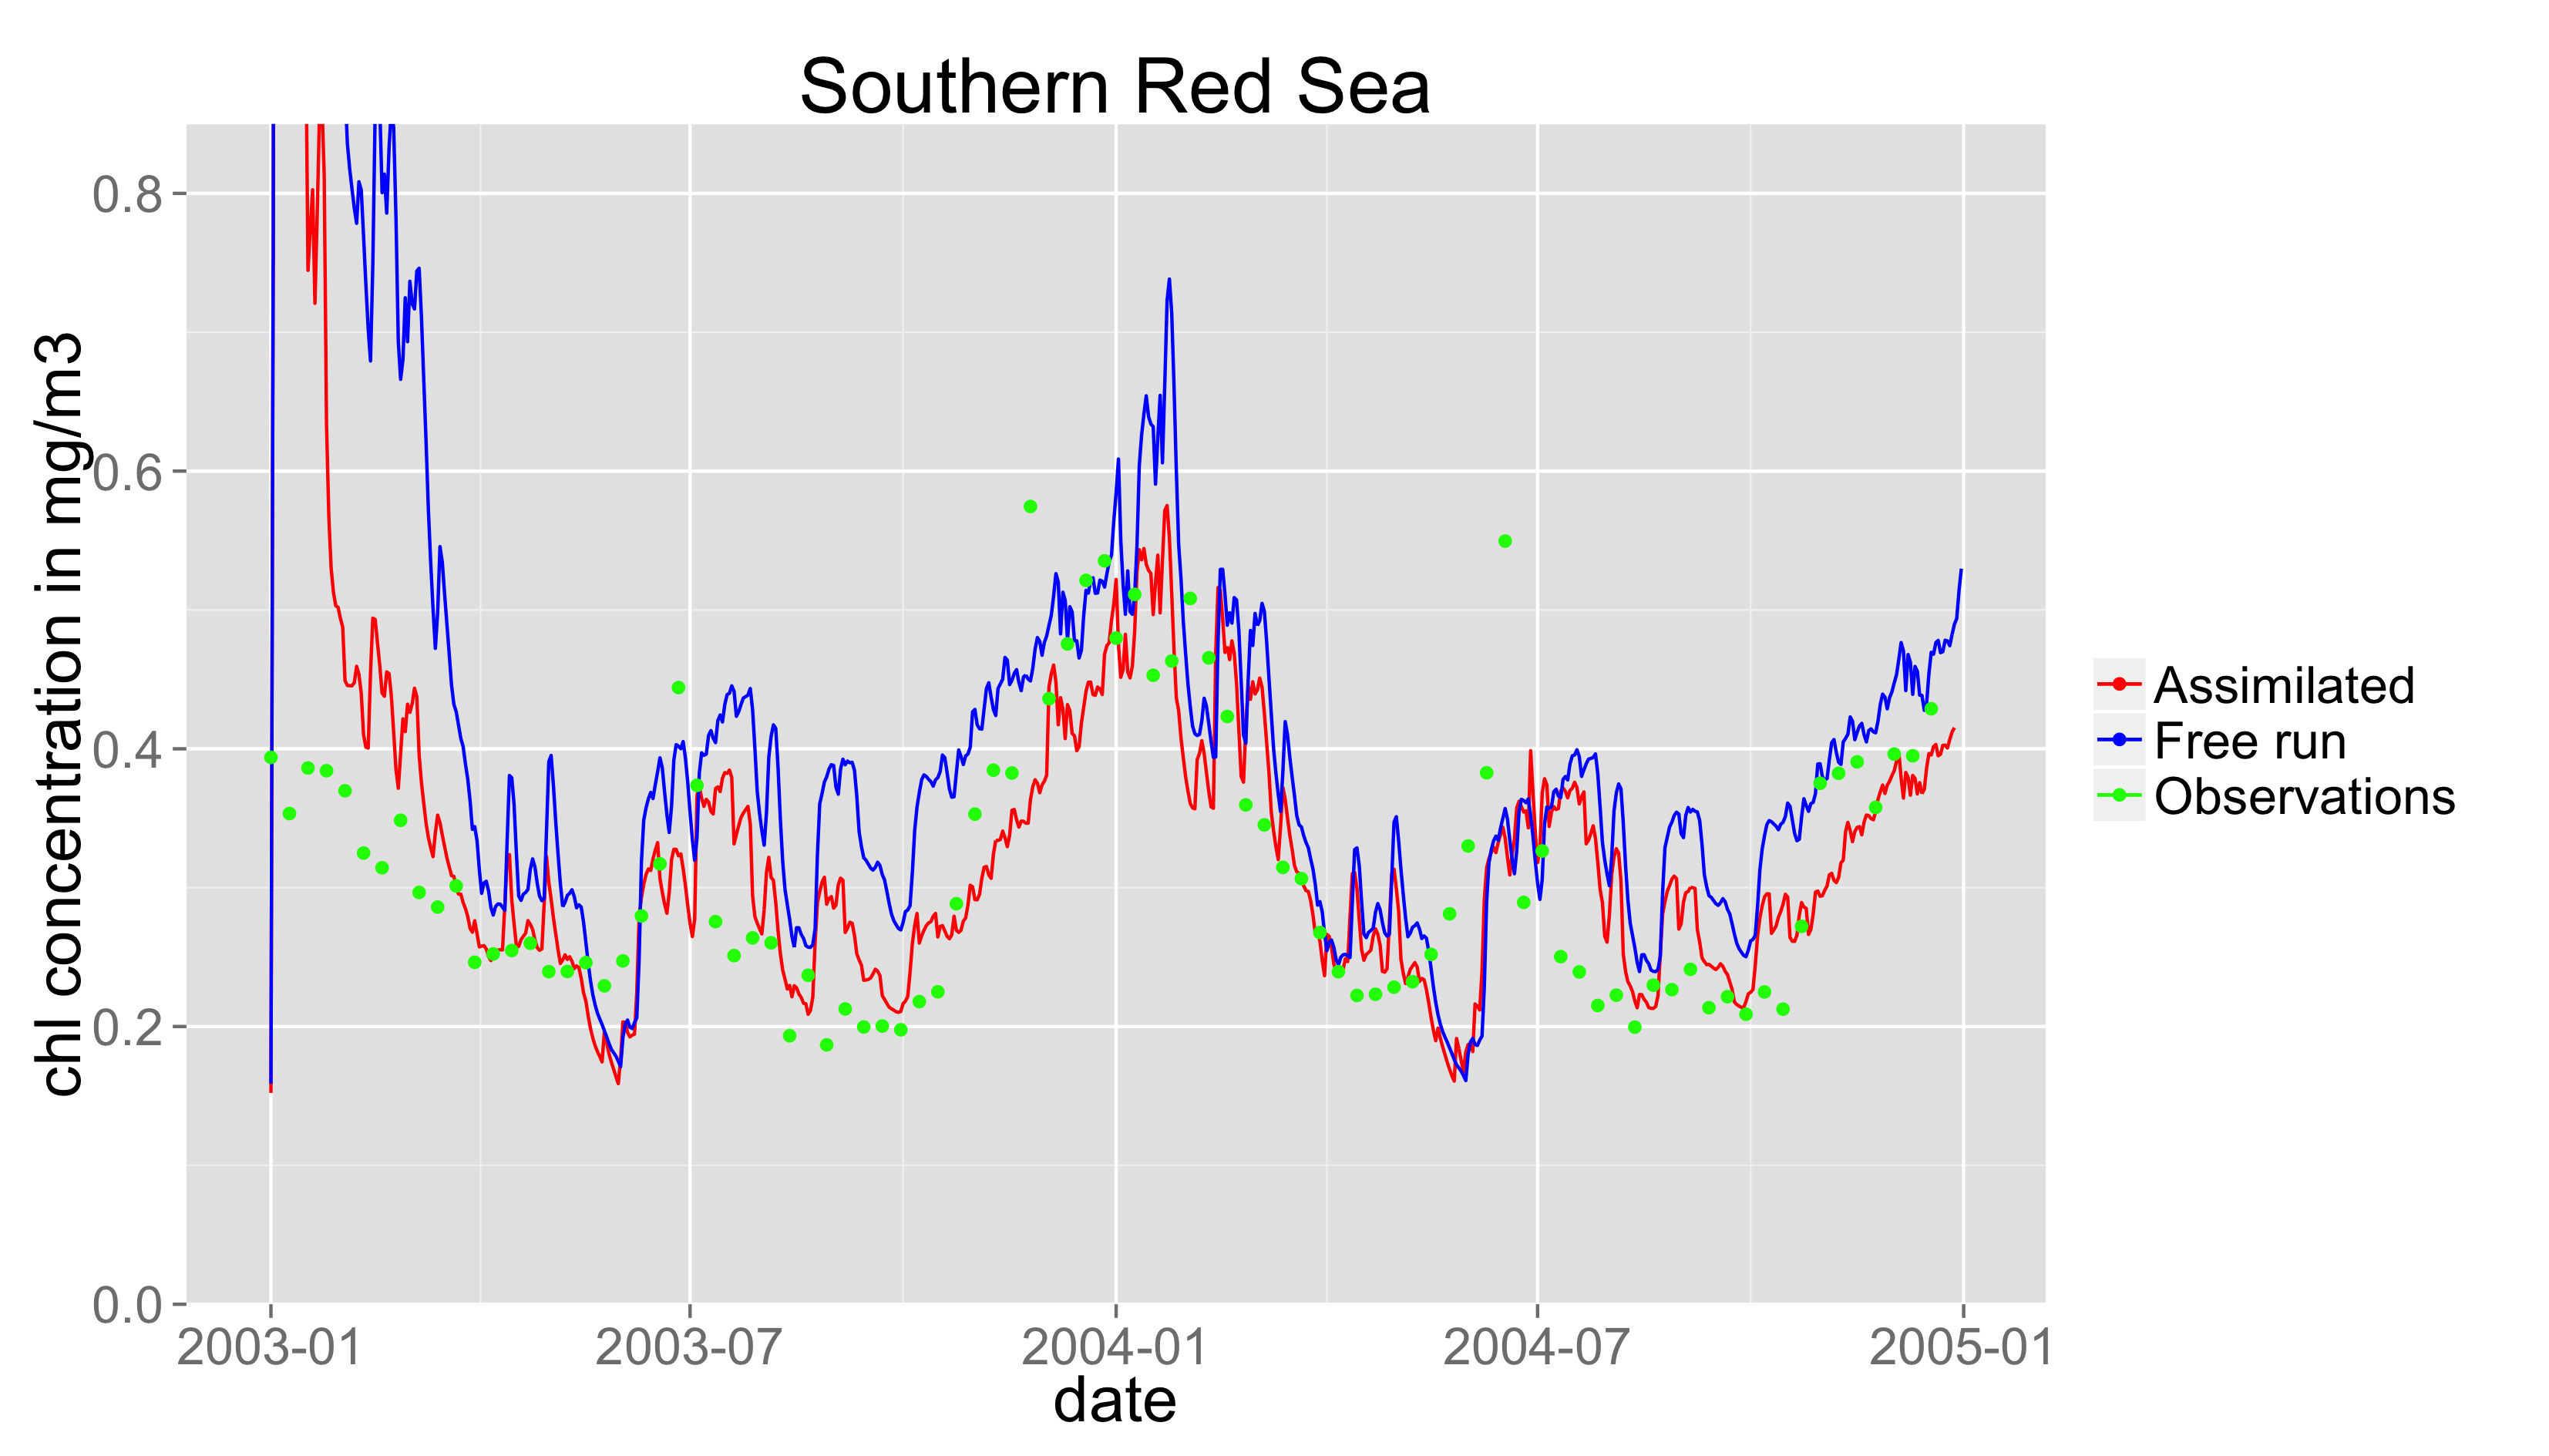
\includegraphics[scale=.15]{figures/chl_models3.png}
    \caption{Surface chlorophyll in the southern Red Sea from CCI data,
             assimilated, and non assimilated 1D ecological model}
    \label{chl_models3}
\end{figure}

The Expectation-Maximization (EM) scheme to estimate the filter parameters has
also been derived. It is similar to that proposed by \citet{Tandeo2014}, which
we generalize to nonlinear models. The scheme will be further extended to estimate
of the observation and model covariance errors. We outline the steps of the EM
scheme hereafter.

\newcommand\x{\mathbf{x}}
\newcommand\y{\mathbf{y}}
\newcommand\eeta{\mathbf{\boldsymbol\eta}}
\newcommand\vvarepsilon{\mathbf{\boldsymbol\varepsilon}}

We consider the state-space system:
\begin{IEEEeqnarray}{rClR}
  \x_k & = & f_k(\x_{k-1}) + \eeta_k,    & k=0,...,K\\
  \y_k & = & h_k(\x_k) + \vvarepsilon_k, & k=1,...,K.
\end{IEEEeqnarray}
The first equation is the state equation, where $\x_k$ is a vector representing
the state of the system (unknown), $f_k$ is the nonlinear model that integrates
the state between time $t_{k-1}$ and $t_k$, and $\eeta_k \sim N(0,Q)$ iid is
the model error. The second equation is the measurement equation, where $\y_k$
is the observation available at time $t_k$, $h$ is the observation operator
that maps the system state to the observation, and $\vvarepsilon_k \sim N(0,R)$
iid is the measurement error. The initial state follows a distribution $\x_0
\sim N(\x_b, B)$.

We use the EM scheme in order to estimate the unknown parameters $Q$, $R$,
$\x_b$, and $B$ that we regroup under the variable $\Theta$. EM is an iterative
procedure to compute the maximum likelihood estimator:
\begin{IEEEeqnarray}{c}
  \Theta_{\text{ML}} = \text{arg}\max(\log p(\y_{1:K}|\Theta)),
\end{IEEEeqnarray}
when it is impossible to analytically express the function to optimize.
$\y_{1:K}$ designates all the observations from time step 1 to time step
$K$.

Given an initial estimate $\Theta^{(0)}$, the following two steps are iterated
until convergence:

\paragraph{Expectation Step:}
The function $G(\Theta) = E_{|\Theta=\Theta^{(r)}}[\log p(\x_{0:K}|\Theta,
y_{1:K})]$ is computed. In the case where $f$ and $h$ are linear, the
distribution can be exactly computed using the Kalman smoother procedure
\citep{Shumway1982}. Otherwise, the distribution can be estimated using, for
example, an ensemble smoother \citep{Tandeo2014}. This is the strategy we
use, since the ecological models are nonlinear.

\paragraph{Maximization Step:}
The function $G$ is maximized to compute a new estimate of the parameters:
\begin{IEEEeqnarray}{c}
  \Theta^{(r+1)} = \text{arg}\max_{\Theta} G(\Theta).
\end{IEEEeqnarray}
EM is guaranteed to converge when $G$ can be exactly computed. Results from
preliminary experiments with a linear system showed that EM may still converge
when using an ensemble smoother.
